\chapter{Ensayos y resultados}

En este capítulo se describen las pruebas realizadas para validar el correcto
funcionamiento del sistema desarrollado. A continuación se detallan los ensayos de hardware, de firmware y de integración,
y finalmente se expone un análisis crítico de los resultados obtenidos.

% ─────────────────────────────────────────────────────────────────
\section{Plan de ensayos}
% ─────────────────────────────────────────────────────────────────
\label{sec:plan_ensayos}
Esta sección describe la metodología de verificación adoptada, los instrumentos
utilizados y los criterios de aceptación que se aplicaron para determinar el éxito
de cada prueba.

\subsection{Metodología}

La estrategia de verificación se organizó en tres etapas sucesivas y dependientes
entre sí. En la primera etapa se realizaron ensayos de hardware sobre cada
componente electrónico de forma individual, con el objetivo de confirmar el
correcto funcionamiento de las señales, los niveles de tensión y la respuesta
eléctrica de cada módulo antes de incorporarlo al sistema. En la segunda etapa
se ejecutaron ensayos de firmware que verificaron el comportamiento de los
módulos de software: la máquina de estados, la gestión de tareas concurrentes
en FreeRTOS y el protocolo de comunicación. En la tercera etapa se realizaron
ensayos de integración con el prototipo completo en operación, donde se
evaluaron los escenarios de uso real del sistema.

Todos los ensayos se realizaron sobre el circuito ensamblado en una placa de
pruebas (\textit{protoboard}) mediante cables de conexión tipo \textit{jumper},
lo que simuló las condiciones del entorno de trabajo previsto.

\subsection{Instrumentos utilizados}

Los instrumentos y herramientas empleados durante los ensayos fueron los
siguientes:

\begin{itemize}
    \item Analizador lógico Saleae~\cite{saleae}, utilizado para la observación de
    señales PWM, I\textsuperscript{2}C y UART.
    \item Multímetro digital, empleado para la medición de tensiones de
    alimentación y verificación de continuidad en el cableado.
    \item Terminal serie (\textit{software}), utilizada para registrar los valores
    transmitidos por el microcontrolador a través del puerto UART.
    \item Masas de referencia calibradas, empleadas para la validación del sistema
    de pesaje.
    \item Aplicación de escritorio desarrollada en Flutter, utilizada como interfaz
    de usuario durante los ensayos de integración.
\end{itemize}

\subsection{Criterios de aceptación}

La tabla~\ref{tab:criterios} resume los criterios de aceptación definidos para
cada prueba. Cada criterio establece la condición mínima que debe satisfacerse
para considerar superado el ensayo correspondiente.

\begin{table}[H]
    \centering
    \caption{Criterios de aceptación por módulo.}
    \label{tab:criterios}
    \begin{tabular}{p{3.5cm} p{8.5cm}}
        \hline
        \textbf{Módulo} & \textbf{Criterio de aceptación} \\
        \hline
        Pesaje (HX711) & Variación máxima inferior a 2~g entre lecturas sucesivas
        sin cambio de carga. \\
        Motor NEMA~17 & Respuesta correcta en todo el rango de velocidades
        ensayado, sin pérdida de pasos. \\
        RTC DS3231 & Conservación de la hora tras un ciclo de apagado, con
        exactitud verificada durante una hora. \\
        Comunicación & Transmisión y recepción de mensajes JSON sin pérdidas
        ni errores de formato. \\
        Pulsador & Generación de exactamente un evento por accionamiento
        válido, sin eventos espurios por rebote. \\
        LED de estado & Comportamiento visual conforme al estado activo de la
        máquina de estados en todo momento. \\
        Integración & Ausencia de condiciones de carrera, bloqueos de tareas
        o pérdida de mensajes durante la operación continua. \\
        \hline
    \end{tabular}
\end{table}

% ─────────────────────────────────────────────────────────────────
\section{Ensayos de hardware}
\label{sec:ensayos_hw}
% ─────────────────────────────────────────────────────────────────

En esta sección se presentan las pruebas realizadas sobre los componentes
electrónicos del sistema. Para cada módulo se documentaron las condiciones
de medición, las señales observadas y los resultados obtenidos.

\subsection{Celda de carga y módulo HX711}

Para verificar el correcto funcionamiento del sistema de pesaje, se conectó la
celda de carga al módulo HX711 y este al microcontrolador STM32F446RE mediante
las líneas CLK y DATA, según lo descrito en la sección~\ref{sec:interconexion_componentes}.
La tensión de alimentación del módulo se verificó con el multímetro y resultó
de 4,98~V, dentro del rango nominal de operación.

La prueba contempló tres escenarios: una lectura sin carga sobre la celda para
verificar la tara, la colocación de una masa de referencia conocida para validar
la respuesta del sistema y una lectura continua durante diez minutos para detectar
deriva en la señal. En la figura~\ref{fig:prueba_hx711} se observa la salida de
la terminal serie durante la lectura continua, donde el campo
\texttt{tank\_weight} refleja el peso registrado por la celda de carga. El valor
se mantuvo estable entre lecturas sucesivas, sin variaciones que excedieran el
criterio de aceptación.

\begin{figure}[H]
    \centering
    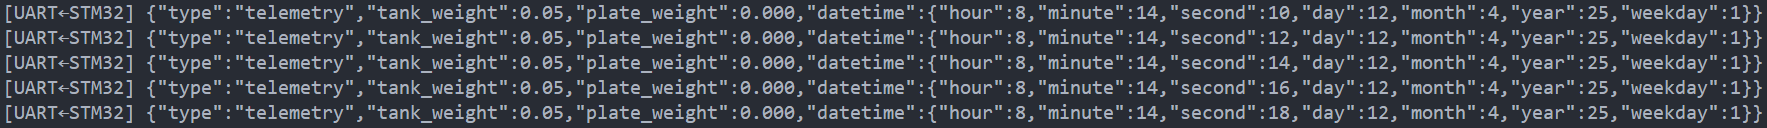
\includegraphics[width=1\textwidth, height=1.5cm]{./Figures/prueba_hx711.png}
    \caption{Lecturas sucesivas del sistema de pesaje registradas en la terminal serie.}
    \label{fig:prueba_hx711}
\end{figure}

Tras la inicialización y la tara, el sistema registró valores estables y coherentes
con la masa de referencia empleada. La variación máxima observada entre
lecturas sucesivas sin cambio de carga fue inferior a 2~g, lo que satisfizo el
criterio de aceptación establecido.

\subsection{Motor paso a paso NEMA~17 y driver A4988}

La verificación del mecanismo de dispensado se realizó sobre el montaje del motor
NEMA~17 con el \textit{driver} A4988, alimentado a 12~V. Con el analizador lógico
se capturó la señal STEP generada por el canal~3 del temporizador TIM2 en modo PWM
sobre el pin PB10, y se verificó que la forma de onda correspondiera a la
frecuencia configurada por \textit{software}. Las señales GPIO DIR y ENABLE se
verificaron con el multímetro, y se confirmaron los niveles lógicos correctos en cada
estado.

Se evaluaron tres condiciones: la rotación en sentido horario y antihorario
mediante el cambio de estado de la señal DIR, la habilitación y deshabilitación
del \textit{driver}, y la variación de la frecuencia de la señal STEP para
comprobar el rango de velocidades.

El motor respondió correctamente en todo el rango de velocidades ensayado.
No se detectó pérdida de pasos ni calentamiento excesivo del \textit{driver}
en operación normal, por lo que se consideró superado el criterio de aceptación
correspondiente.

\subsection{Módulo RTC DS3231}

Para evaluar el módulo de reloj de tiempo real, se estableció la comunicación
I\textsuperscript{2}C entre el STM32F446RE y el DS3231 mediante las líneas SCL
y SDA del periférico I\textsuperscript{2}C1, configurado a 400~kHz. Las señales del bus se verificaron con el analizador lógico Saleae. Los niveles lógicos y los tiempos de establecimiento  se encontraron dentro de las especificaciones del protocolo.

Se comprobaron los siguientes aspectos:

\begin{itemize}
    \item La escritura y lectura correcta de fecha y hora en los registros del \mbox{dispositivo}.
    \item La conservación de la hora tras un ciclo de apagado, con la batería de
    respaldo CR1220 desconectada del circuito principal.
    \item La exactitud de la temporización comparada con una referencia externa
    durante un período de observación de una hora.
\end{itemize}

La figura~\ref{fig:prueba_rtc} presenta la
captura del analizador lógico sobre el bus I\textsuperscript{2}C durante una
lectura del DS3231. Se observa la dirección del dispositivo (0x68) en las
operaciones de escritura y lectura, junto con los registros de fecha y hora
codificados en BCD. El último byte se transmite con un NAK del maestro, lo que
corresponde al cierre normal de una lectura I\textsuperscript{2}C y confirma el
cumplimiento del protocolo.

\begin{figure}[H]
    \centering
    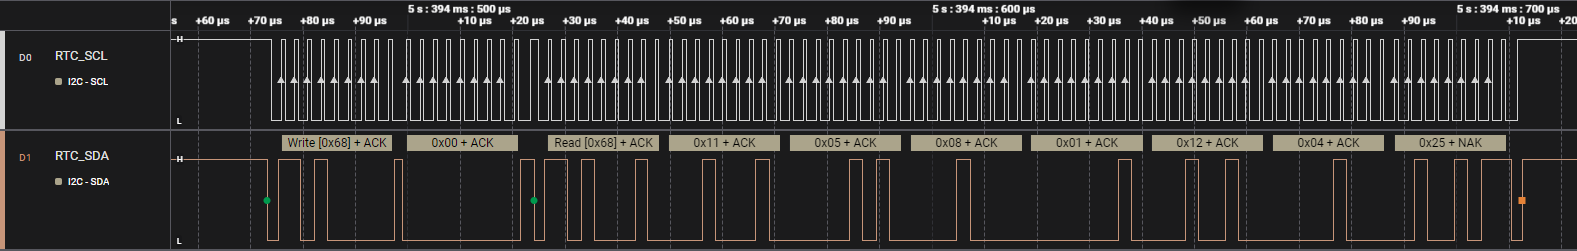
\includegraphics[width=\textwidth, height=3cm]{./Figures/prueba_rtc.png}
    \caption{Captura del bus I\textsuperscript{2}C entre el STM32 y el DS3231 obtenida con el analizador lógico.}
    \label{fig:prueba_rtc}
\end{figure}

Los datos de fecha y hora se leyeron correctamente en todos los ciclos. La hora
se conservó tras la desconexión de la alimentación principal, lo que confirmó
el correcto funcionamiento de la batería de respaldo.

\subsection{Pulsador de dispensado manual}

Para validar el pulsador, se configuró el pin de entrada del STM32F446RE con
interrupción externa (EXTI). Con el analizador lógico se capturó la señal en el pin
de entrada durante el accionamiento, lo que permitió caracterizar el rebote
mecánico del contacto y confirmar que el tiempo de antirrebote de 200~ms
implementado por \textit{software} resultó suficiente para suprimirlo.

Se registraron 50 pulsaciones consecutivas en diferentes intervalos de tiempo.
En todos los casos se generó exactamente un evento de interrupción por
accionamiento sin eventos espurios, lo que satisfizo el criterio de aceptación
definido.

\subsection{LED de estado del sistema}

La prueba del LED de estado consistió en verificar con el multímetro la tensión
sobre el componente en cada estado de la máquina de estados. Se comprobó
que el LED permaneciera encendido de forma continua en el estado
\texttt{ST\_ERROR}, parpadeara a 1~Hz en el estado \texttt{ST\_IDLE} y se
apagara en el estado \texttt{ST\_DISPENSING}. Todos los patrones de iluminación
respondieron conforme a lo especificado.

% ─────────────────────────────────────────────────────────────────
\section{Ensayos de firmware}
\label{sec:ensayos_fw}
% ─────────────────────────────────────────────────────────────────

En esta sección se presentan las pruebas de las funciones de \textit{software}:
el comportamiento de la máquina de estados, la gestión de tareas concurrentes
bajo FreeRTOS y el protocolo de comunicación, junto con la verificación del
\textit{timing} de los mensajes de telemetría.

\subsection{Máquina de estados y módulo orquestador}

Se verificó el comportamiento de la máquina de estados finita implementada
en el módulo orquestador, descripta en la sección~\ref{sec:modulo_orquestador},
mediante la ejecución de transiciones forzadas entre estados. Para cada
transición se registró por la terminal serie el estado de origen, el evento
disparador y el estado de destino, y se compararon los resultados con el
diagrama de la figura~\ref{fig:estados}.

La tabla~\ref{tab:fsm_prueba} resume los casos de prueba ejecutados y los
resultados obtenidos.

\begin{table}[H]
    \centering
    \caption{Resultados de las pruebas unitarias de la máquina de estados.}
    \label{tab:fsm_prueba}
    \begin{tabular}{>{\ttfamily}p{3.0cm} p{4.3cm} >{\ttfamily}p{3.2cm} c}
        \hline
        \textnormal{\textbf{Estado inicial}} & \textbf{Evento}
        & \textnormal{\textbf{Estado esperado}} & \textbf{Resultado} \\
        \hline
        ST\_INIT & Inicialización exitosa & ST\_IDLE & OK \\
        ST\_INIT & Error irrecuperable & ST\_ERROR & OK \\
        ST\_IDLE & \texttt{EVT\_BUTTON} & ST\_DISPENSING & OK \\
        ST\_IDLE & \texttt{EVT\_SCHEDULED\_FEED} & ST\_DISPENSING & OK \\
        ST\_DISPENSING & Dispensado completo & ST\_IDLE & OK \\
        ST\_ERROR & Reinicio tras 10~s & ST\_INIT & OK \\
        \hline
    \end{tabular}
\end{table}

Todos los casos de prueba produjeron las transiciones esperadas. El mecanismo
de inhibición que evita disparos múltiples dentro de la misma ventana temporal
de un minuto también fue verificado y respondió correctamente.

\subsection{Gestión de tareas concurrentes en FreeRTOS}

Se verificó la correcta convivencia de las dos tareas principales del firmware:
la tarea de control del dispensado y la tarea de comunicación. Para ello se
ejecutó el sistema durante un período prolongado con dispensados automáticos
programados cada cinco minutos, mientras la tarea de comunicación transmitía
mensajes de telemetría de forma continua.

Se comprobó que la cola de mensajes \texttt{xQueueHandle} cumplió su función
de sincronización entre ambas tareas, sin pérdida de eventos ni bloqueos. Durante todo el período de observación, el planificador de FreeRTOS ejecutó ambas
tareas con regularidad, sin que ninguna dejara de recibir tiempo de procesamiento.

\subsection{Protocolo de comunicación y \textit{timing} de telemetría}

Se verificó el protocolo de comunicación JSON entre el microcontrolador y la
aplicación de escritorio. Para ello se conectó el ESP32 al STM32 mediante UART4,
configurado a 115\,200 baudios con formato 8N1, y se registraron los mensajes
intercambiados durante una sesión de uso mediante el monitor serie de PlatformIO.

El protocolo contempla tres mensajes salientes del microcontrolador hacia la
aplicación y tres comandos entrantes desde la aplicación. Los mensajes salientes
son la telemetría periódica, la confirmación de dispensado y la confirmación de
tara. Los comandos entrantes son el dispensado manual, la actualización de horarios
y la tara remota.

La figura~\ref{fig:prueba_bt} muestra el registro obtenido en el monitor serie de
PlatformIO durante una sesión de comunicación. Se observa la recepción del comando
\texttt{set\_\allowbreak schedules} con la lista de horarios enviada desde la aplicación, la
confirmación de su recepción por parte del firmware y los mensajes de telemetría
transmitidos de forma periódica, cada uno con los valores de peso y la marca
temporal correspondientes.

\begin{figure}[H]
    \centering
    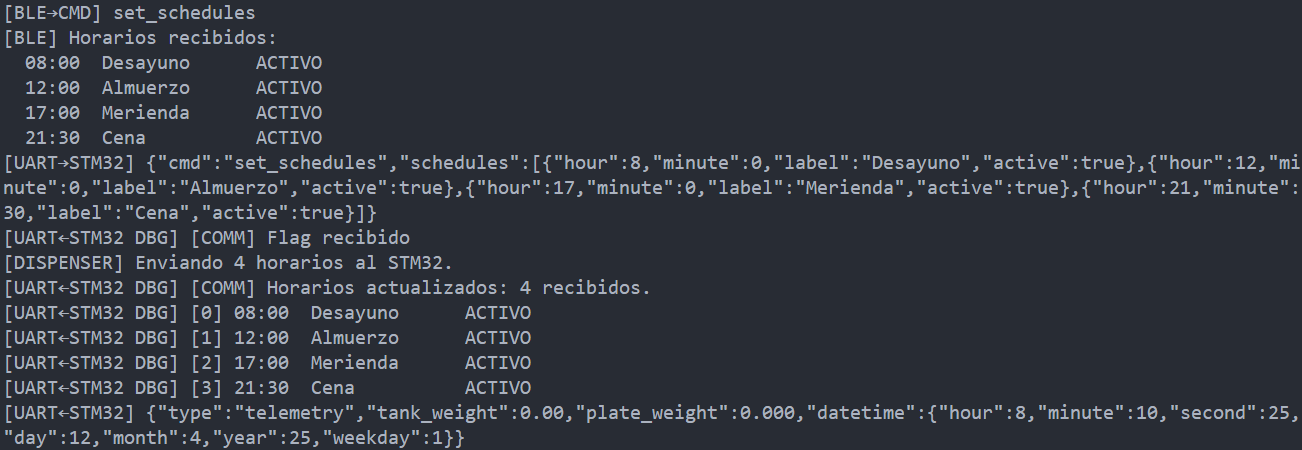
\includegraphics[width=\textwidth]{./Figures/prueba_bt.png}
    \caption{Registro de la comunicación JSON entre la aplicación y el microcontrolador.}
    \label{fig:prueba_bt}
\end{figure}

El período entre mensajes de telemetría consecutivos se midió con una referencia
temporal externa y resultó de 1,00~s ± 0,02~s, conforme a lo especificado. No
se detectaron pérdidas de mensajes ni errores de formato en los datos
intercambiados durante las pruebas.

% ─────────────────────────────────────────────────────────────────
\section{Ensayos de integración}
\label{sec:ensayos_integracion}
% ─────────────────────────────────────────────────────────────────

En esta sección se presentan las pruebas del sistema completo con todos los
módulos interconectados y el firmware operando bajo FreeRTOS. Se describen
los escenarios evaluados y los resultados obtenidos.

Una vez superadas las pruebas individuales, se procedió a la integración del
sistema completo sobre la \textit{protoboard}, con todos los componentes
interconectados según el esquema de la sección~\ref{sec:interconexion_componentes}.

La tabla~\ref{tab:integracion} resume los escenarios evaluados, el resultado
esperado y el resultado obtenido para cada caso.

\begin{table}[H]
    \centering
    \caption{Resultados esperados vs. obtenidos en los ensayos de integración.}
    \label{tab:integracion}
    \begin{tabular}{p{5.5cm} p{5.5cm} c}
        \hline
        \textbf{Escenario} & \textbf{Resultado esperado} & \textbf{Resultado} \\
        \hline
        Dispensado automático por horario programado &
        Activación del motor y envío de mensaje \texttt{feeding\_done} &
        Conforme \\
        Dispensado manual por pulsador físico &
        Activación del motor y envío de mensaje \texttt{feeding\_done} &
        Conforme \\
        Monitoreo de telemetría en tiempo real &
        Recepción de mensaje cada 1~s con pesos actualizados &
        Conforme \\
        Tara remota desde la aplicación &
        Tara ejecutada y confirmada por terminal &
        Conforme \\
        Actualización de horarios desde la aplicación &
        Nuevos horarios almacenados en \textit{flash} y activos &
        Conforme \\
        Corte y restitución de alimentación eléctrica &
        Hora conservada en el DS3231 y sistema retomado &
        Conforme \\
        \hline
    \end{tabular}
\end{table}

La figura~\ref{fig:app_integracion} ilustra la interfaz de la aplicación durante
los ensayos de integración. Se muestran la confirmación de la vinculación
Bluetooth (figura~\ref{fig:app_vinculacion}), la configuración de horarios cargada
en el dispositivo (figura~\ref{fig:app_horarios}) y la pantalla principal durante
el monitoreo en tiempo real (figura~\ref{fig:app_monitoreo}), donde se observan
los pesos del tanque y del plato junto con el registro de la última alimentación.

\begin{figure}[H]
    \centering
    \begin{subfigure}[t]{0.32\textwidth}
        \centering
        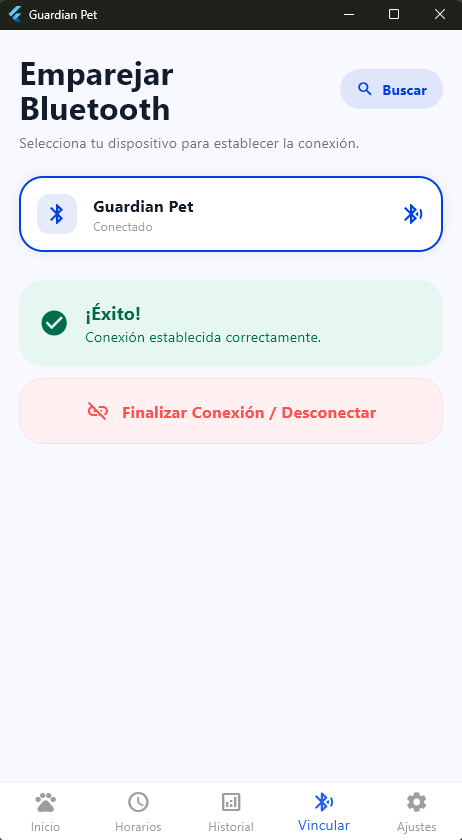
\includegraphics[width=\textwidth]{./Figures/app_vinculacion.png}
        \caption{Vinculación Bluetooth.}
        \label{fig:app_vinculacion}
    \end{subfigure}
    \hfill
    \begin{subfigure}[t]{0.32\textwidth}
        \centering
        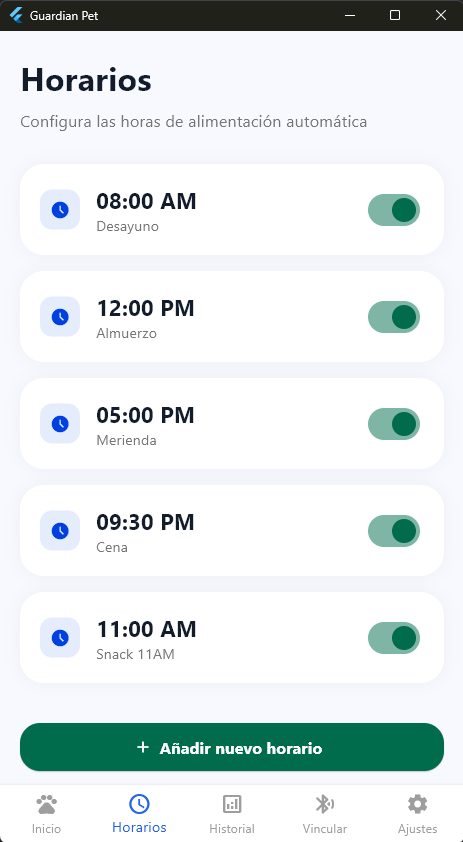
\includegraphics[width=\textwidth]{./Figures/app_horarios.png}
        \caption{Configuración de horarios.}
        \label{fig:app_horarios}
    \end{subfigure}
    \hfill
    \begin{subfigure}[t]{0.32\textwidth}
        \centering
        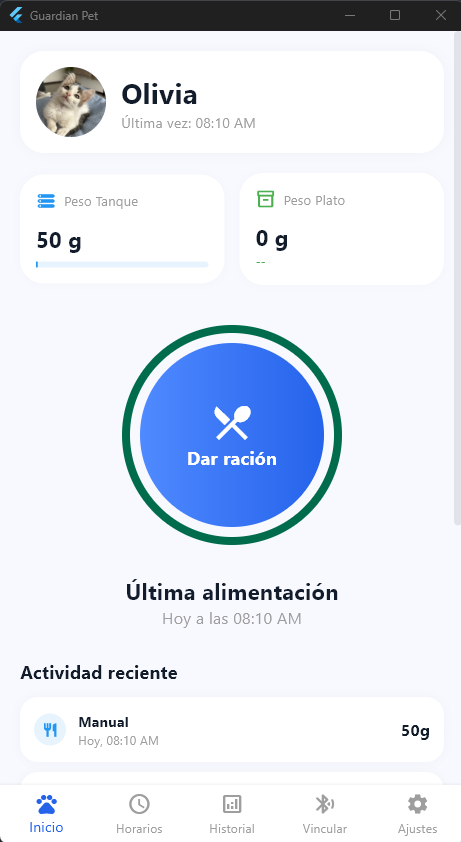
\includegraphics[width=\textwidth]{./Figures/app_integracion.png}
        \caption{Monitoreo en tiempo real.}
        \label{fig:app_monitoreo}
    \end{subfigure}
    \caption{Interfaz de la aplicación durante los ensayos de integración.}
    \label{fig:app_integracion}
\end{figure}

El sistema respondió correctamente en todos los escenarios evaluados. La
comunicación Bluetooth no presentó interrupciones, los eventos de dispensado
se registraron con la hora correcta provista por el DS3231, y el pesaje del plato
permitió detectar la variación de masa producida por el alimento dispensado.

% ─────────────────────────────────────────────────────────────────
\section{Análisis de resultados}
\label{sec:analisis_resultados}
% ─────────────────────────────────────────────────────────────────

En esta sección se analizan los resultados obtenidos en las etapas anteriores,
se identifican las limitaciones observadas y se explican los desvíos detectados
respecto de lo especificado.

\subsection{Cumplimiento de criterios de aceptación}

Todos los criterios de aceptación definidos en la sección~\ref{sec:plan_ensayos}
y resumidos en la tabla~\ref{tab:criterios} se cumplieron satisfactoriamente.
El sistema de pesaje alcanzó la resolución requerida de 2~g,
el motor operó sin pérdida de pasos en el rango de velocidades previsto, la hora
se conservó ante cortes de energía, y la comunicación JSON no presentó errores
en ninguna de las sesiones de prueba.

\newpage
\subsection{Limitaciones identificadas}

Durante los ensayos se identificaron las siguientes limitaciones del prototipo:

\begin{itemize}
    \item La resolución del sistema de pesaje de 2~g resulta adecuada para
    detectar el consumo de raciones mayores a 10~g, pero puede ser insuficiente
    para raciones pequeñas o para monitorear el consumo de agua en futuras
    versiones del dispositivo.
    \item El alcance efectivo del enlace Bluetooth Classic en el entorno de prueba
    fue de aproximadamente 8~m en línea de visión directa, lo que podría
    representar una limitación en viviendas de gran superficie.
    \item El ensamblado sobre \textit{protoboard} con cables \textit{jumper}
    introduce capacitancias parásitas y resistencias de contacto que no estarían presentes en un diseño con placa de circuito impreso (PCB), por lo que los
    resultados de consumo de corriente deben interpretarse como valores
    aproximados.
\end{itemize}

\subsection{Desvíos respecto de lo planificado}

El único desvío identificado respecto de lo especificado originalmente fue la
variabilidad en el período de telemetría, que presentó una dispersión de
±0,02~s en lugar del valor nominal de 1~s exacto. Este desvío se atribuyó a la
latencia introducida por el planificador de FreeRTOS al momento de despertar la
tarea de comunicación, y no representa un inconveniente para la aplicación
prevista, dado que el usuario percibe la actualización como continua.
